\section{Introduction}

One of the present challenges in cybersecurity systems is to outsource programs to be executed in the cloud and at the same time maintaining the privacy of the owner and the security of data. The program code has to be protected alongside the data which is being used inside it. Even in a securely encrypted code, the low-level instructions are visible when they are being executed by the CPU and a malicious operating system kernel can tamper with them. Several attacks are possible by reverse engineering the instructions, including code reuse, data injection, copyright violation, and recovery of classified data. Intel SGX (Software Guard eXtensions) \cite{sgx} is a novel architecture introduced with Intel Skylake micro-architecture \cite{skylake} that protects the code and the data inside an encrypted enclave that is a portion of memory which is protected by the support of hardware. The enclave is secure against direct eavesdropping by the adversary, but there are several successful attacking methods using side-channel information which is visible to the adversary \cite{leakycauldron}. The problem with this hardware extension is that the memory layout is still visible to the operating system kernel and a malicious OS in the cloud can recover useful information by observing the occurrences of page faults. As a result, this side-channel attack can be successful on recovering the data by clearing the page table and causing page faults and observing them for different inputs. In the same scenario, cache-misses are a point for side-channel attacks. The pattern of cache-miss occurrences can be used by a malicious operating system to attack the enclave program.

Several theoretical and practical attacks based on SGX side channels discussed and experimented to be practical and effective. The points of interest during the execution of a program inside enclave for the adversary are cache and whatever is missed and retrieved from the memory, page-faults, and page-table which is attacked by making use of accessed and modified bits.

In response to the development of attacks, several defense mechanisms are designed which have been effective in some cases and conditions. These defense methods usually sacrifice performance or accuracy while improving the security against side-channel attacks. 

In this report, we study the possible attacks which are possible using SGX side-channel information and their points of success. Then, we discuss possible defenses which have been proposed by the researchers and study their methods and compare the defenses and their effectiveness under different conditions and scenarios.

In summary, the main points of study in this work are:
\begin{itemize}
	\item Examining SGX enclave points of attacks.
	\item Discussing the past work which have been done on defending the SGX enclave against side-channel attacks.
	\item Comparing and analyzing the defense methods and their effectiveness.
\end{itemize} 
\textbf{Outline} In the remainder of this report, we discuss basic background knowledge required for studying this work in section 2. Then, we review and analyze the attacks which are possible to be launched against SGX enclave using side-channel information in section 3. In section 4, we introduce several defenses which have been proposed by past researches and in section 5 we analyze and compare the effectiveness of these defense methods in terms of security and performance. At last, we conclude the research in section 6.
\section{Background}
In this section, we provide detailed background on side-channel attacks targeting enclaved applications, tools, and terms we use in this report.

\subsection{Intel SGX}

Protecting the data inside a shield has been a major interest for improving security and privacy in distributed systems and several software-based and hardware-based solutions have been proposed for this purpose.

Intel introduced a new hardware-based technique in its new Skylake micro-architecture \cite{skylake} line of processors called Software Guard eXtensions (SGX) \cite{sgx}. The main function of it is assigning a portion of main memory to a program and protect it from being read and written by other processes. The effectiveness of this technique scales up to preventing the operating system kernel itself from accessing the shielded memory which is called enclave. Intel SGX API \cite{sgxapi} uses two main kinds of specialized function calls to work with enclave. ECALLs are functions which run inside the enclave and can be called from outside and OCALLs are useful for using system functions and other operations which are possible to be done outside enclave \cite{ecallocall}.

One of the major problems with running applications inside the cloud is the leakage of data and code instructions. Even with encryption, the CPU can only execute unencrypted instructions which can be eavesdropped and reverse engineered to useful code. Only with hardware modifications and adding SGX support to the hardware, it is possible to improve security and privacy in this term.

\subsection{Storage Structure}

In the common hardware architectures used in cloud computing environments today, data is transferred through several buses using multiple protocols to be used. The encrypted data is stored on the hard drive and will be transferred into enclaved memory. The encrypted data in the main memory will be cached using multiple levels of cache for performance optimization. Also, page mappings between virtual and physical addresses of data are kept in the main memory and a transaction look-aside buffer (TLB) is used to cache the mappings in the page-table for better performance.

Each data transfer can be a point of side-channel attack. While the data is encrypted, the patterns of reads and writes, cache-misses, page-faults, and other interrupts and exceptions can be used by the adversary for launching attacks and recovering useful information.

\subsection{Side-Channel Attacks on the Enclave}

Multiple effective attacks and defenses on the enclave have been proposed by past research. Most of the attacks make use of the side-channel information that can be leaked and accessed by a modified malicious kernel. In these attacks, the malicious kernel retrieves useful information about the code and the data by changing the behavior of program execution or analyzing the page-faults and other possible points of data leakage.

One of the major points of attacks is targeting exceptions caused by the program. Since the exceptions are first acknowledged by the kernel before the program, a malicious OS can use them to infer activities and the behavior of the program according to the inputs which leads to recovering the actual data and code of the program.

Another kind of attack that can be triggered by a malicious OS is an interrupt-based attack. The kernel can trigger interrupts to control the execution of program.

Other attacks such as Stealthy Page Monitoring (SPM) attacks \cite{stealthy,leakycauldron} can also be effective. For a typical page-fault attack, the attacker can make all the page table entries invalid and restrict enclave program’s access to all the pages and by causing page-faults, view the pattern of memory reads and writes by the program. This action will cause a lot of page-faults which lead to a high overhead which leads to attack detection by the victim, so the attacker is interested to retrieve this information and view the pattern without causing unwanted page-faults by the victim. In page monitoring attacks, the attacker monitors the bits representing the validity and whether a page is accessed or modified. The attacker is also able to clear these bits and view them again frequently. So, the pattern of accesses can be visible to the attacker without causing page-faults \cite{stealthy,leakycauldron}.

\begin{figure}
	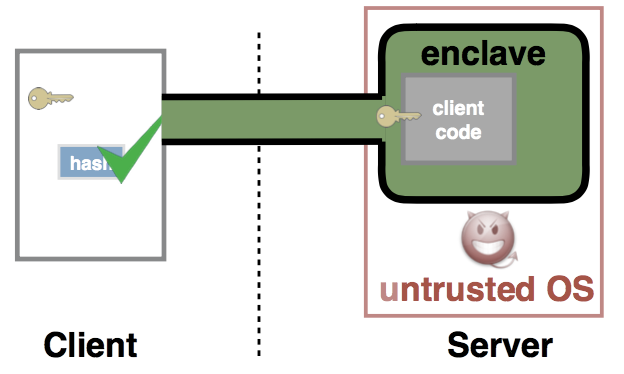
\includegraphics[scale=0.3]{images/uos}
	\caption{Overview of remote attestation available in Intel SGX \cite{wang2017}.}
	\label{fig:uos}
\end{figure}

\begin{figure}
	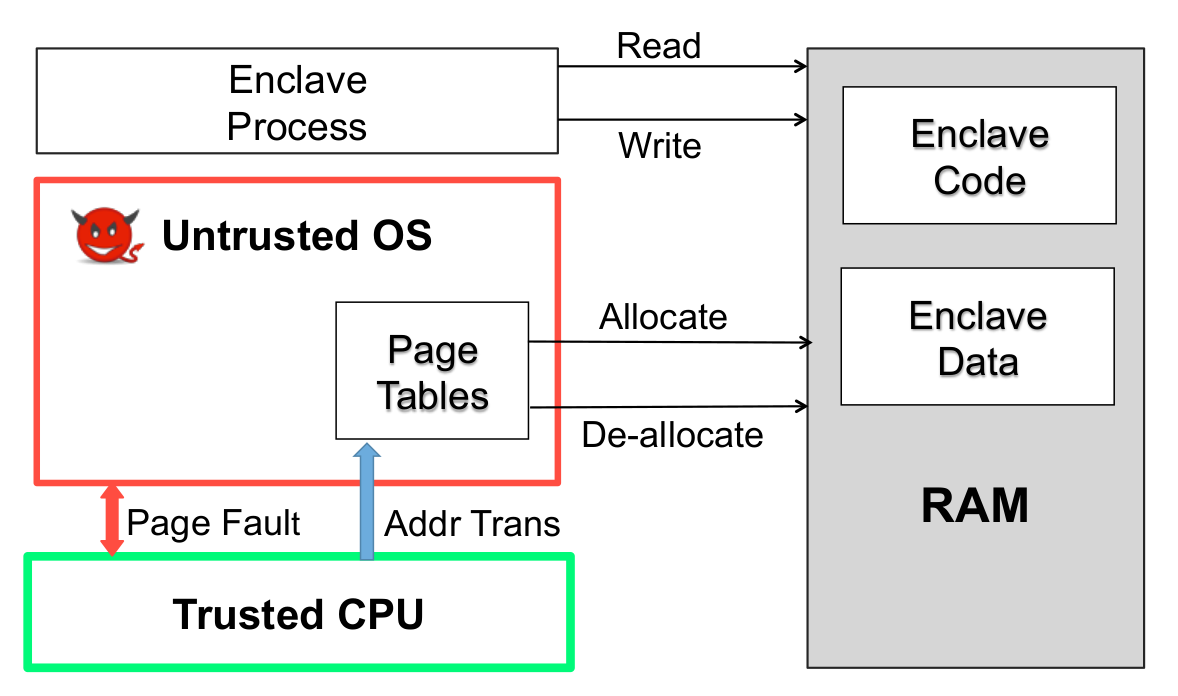
\includegraphics[scale=0.3]{images/uos1}
	\caption{Problem Setting. Process executing in an enclave on untrusted OS \cite{pigeonhole}.}
	\label{fig:uos}
\end{figure}

\subsection{Intel TSX}
One of the technologies which have been came into notice for making benefit in defense against side-channel attacks is Intel TSX \cite{tsx}. This technology has been introduced by Intel since Haswell mirco-architecture \cite{haswell} for critical sections management and monitoring serialization. Intel TSX provides two frameworks to add transaction support to the processor. Both frameworks intoduce new instructions for region specification, backward compatiblity, and flexiblity \cite{tsx}. We use RTM (Restricted Transactional Memory) \cite{rtm} for implementing our defenses in this work.

RTM has been used by previous researches like T-SGX \cite{tsgx} to isolate instructions and Cloak \cite{cloak} to pin sensitive code and data to the caches which is not supported by current hardware instructions.

%We use RTM transactions to detect attacks against the executing program inside enclave. By using RTM, we detect page-faults, interrupts and other unusual behavior performed by the attacker and we can terminate if we guess we are being attacked.

\begin{figure}
	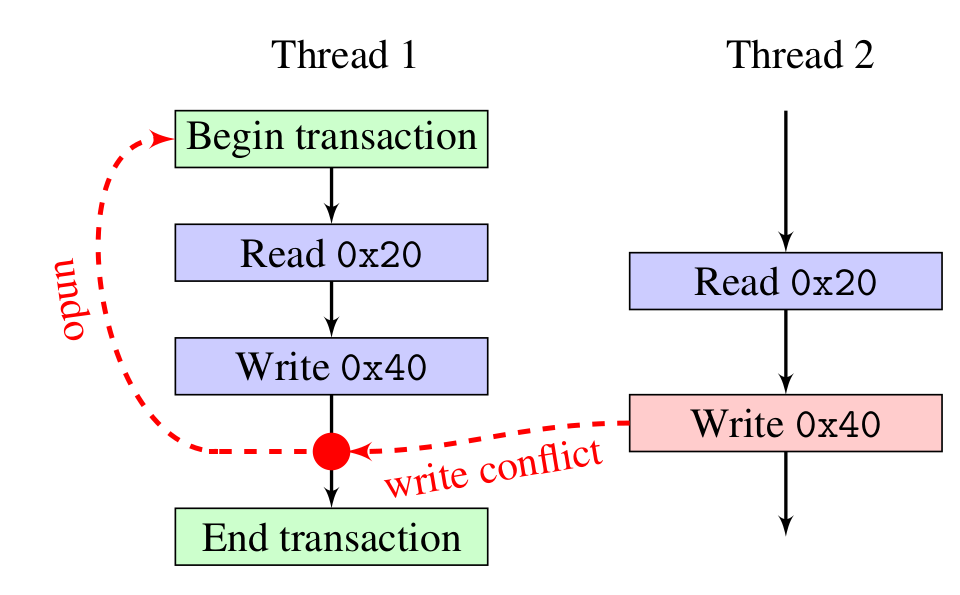
\includegraphics[scale=0.2]{images/rtm}
	\caption{HTM ensures that no concurrent modifications influence the transaction, either by preserving the old value or by aborting and reverting the transaction. \cite{cloak}.}
	\label{fig:rtm}
\end{figure}


\section{Attacks}
Several side-channel attacks on the enclave have been proposed by the past research. Focusing on the thorough work done by Wang et al. \cite{leakycauldron} we focus on summarizing the attacks and the points of attacks in this section.

\subsection{Attack Model}
In our attack scenario, the enclave is protected by Intel SGX, so no one except the main program running inside enclave has the key to access the enclave. The operating system kernel which runs on top of a hypervisor can view and manage tasks queue, exceptions and interrupts. The hypervisor kernel is also capable of viewing data transfer between memories and caches while Intel SGX prevents it from accessing the enclave data. It is considered that other tenants executing on the same hypervisor are not able to control the resources assigned to the main machine by the hypervisor.

\subsection{Points of Attack}
Several weaknesses in SGX architecture have been proposed to be points for launching attacks against the enclave.

TLB, as an address translation cache, can be one point of attack. While TLB is shared between enclave and non-enclave programs when hyper-threading is enabled, it can create side-channels which can be used for retrieving useful information \cite{leakycauldron}.

Also, during AEX (Asynchronous EXit), TLB and paging-structure caches will be flushed and let the adversary know the flushed entries at context switch \cite{leakycauldron}.

Another point of attack is the use of page table entry flags. The accessed and dirty bits which are set and unset for page table entries upon accesses and modifications, are used for launching attacks. So, the code in non-enclave mode can observe page-table updates and the memory write pattern to recover useful data \cite{leakycauldron,stealthy}.

Other than TLBs, CPU caches are shared between the enclave and non-enclave code resulting in the possiblity of cache side-channel attacks \cite{leakycauldron}.

\subsection{Prime+Probe}
Prime+Probe is composed of two stages. Considering an L1 cache of 64 sets, each containing 8 cache lines which are each 64 bytes, in the prime stage, the attacker executes conflicting cache lines to make page fault possible for the victim who branches on a secret. In the probe step, the attacker executes all the cache lines and measures the execution time of each, and if a cache line execution takes longer, it can be revealed that the secret has been zero \cite{primeprobe1,primeprobe2,cloak}.

\begin{algorithm}[t]
	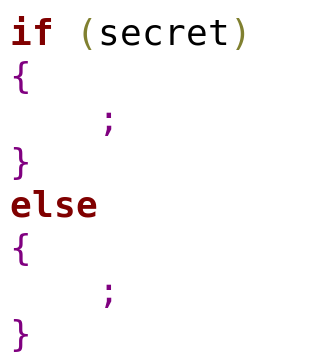
\includegraphics[scale=0.25]{images/alg}
%	\SetAlgoNoLine
%	if ($secret$)
%	\\\{\\
%	\tab ;\\
%	\}\\
%	else\\
%	\{\\
%	\tab;\\
%	\}
	\caption{Prime+Probe branching side-channel sample code \cite{stealthy,cloak}}
	\label{alg:one}
\end{algorithm}

\begin{figure}
	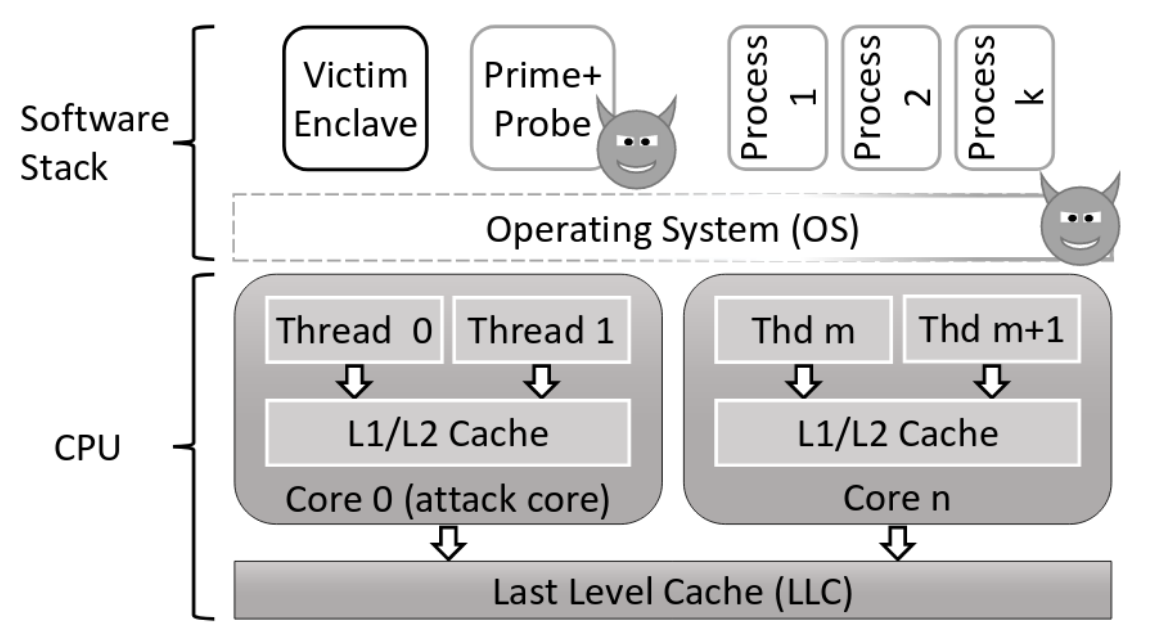
\includegraphics[scale=0.2]{images/pp1}
	\caption{High-level view of our attack; victim and attacker’s Prime+Probe code run in parallel on a dedicated core. The malicious OS  ensures  that  no  other  code shares that core minimizing noise in L1/L2 cache \cite{brasser2017software}.}
	\label{fig:ppone}
\end{figure}
\begin{figure}
	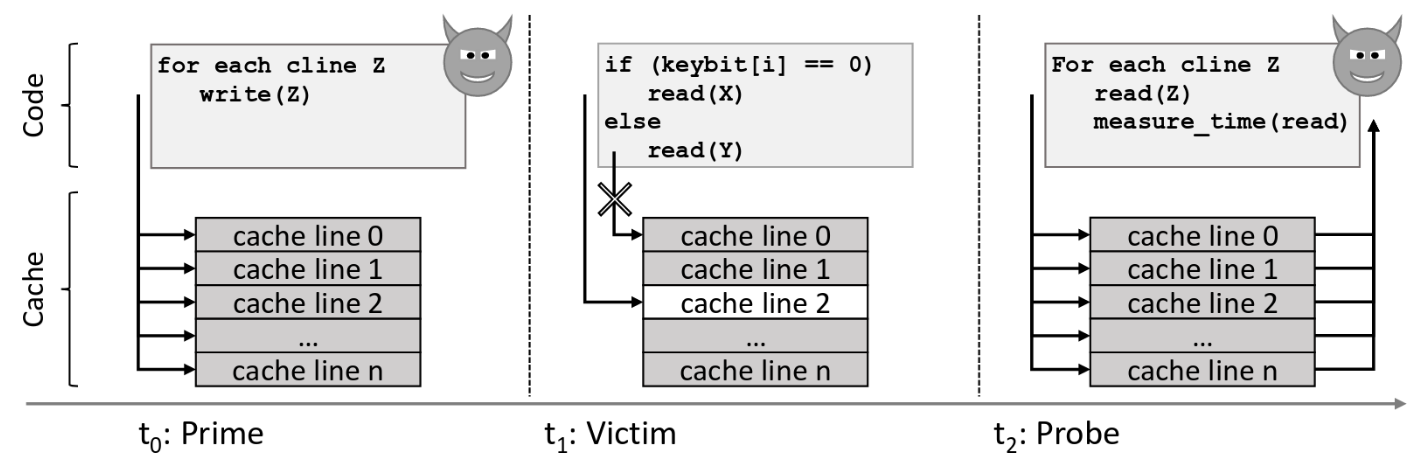
\includegraphics[scale=0.2]{images/pp2}
	\caption{Prime+Probe side-channel attack technique; first the attacker primes the cache, next the victim executes and occupies some of the cache, afterwards the attacker probes to identify which cache lines have been used by the victim. This information allows the attacker to draw conclusion on secret data processed by the victim process \cite{brasser2017software}.}
	\label{fig:pptwo}
\end{figure}
\begin{figure}
	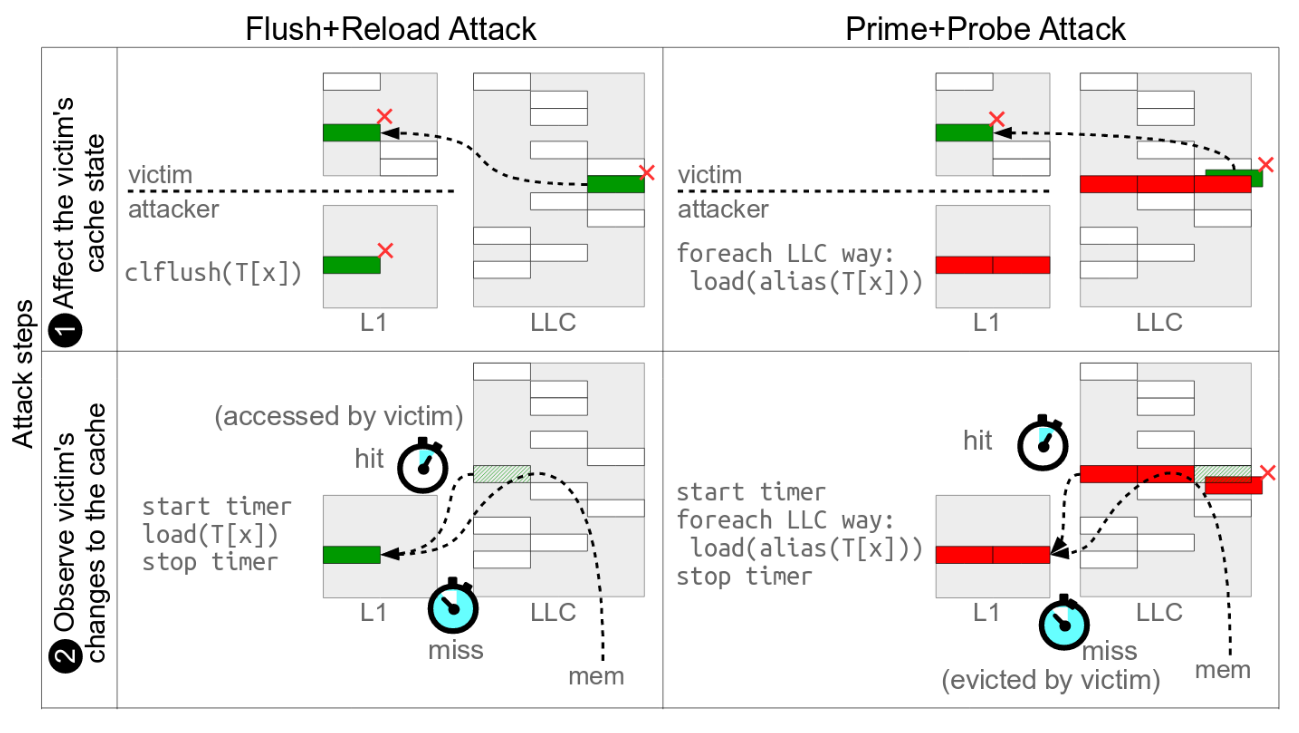
\includegraphics[scale=0.2]{images/ppfr}
	\caption{Prime+Probe vs Flush+Reload Attacks \cite{kayaalp2016high}.}
	\label{fig:ppfr}
\end{figure}

\subsection{Flush+Reload}
By making use of page sharing between enclave and non-enclave code, the attacker can find out if a certain page is removed from the cache. More precisely, the attacker flushes the target memory line from the cache and waits for the victim to access it. The wait time can be fixed to either a random value or a value that is experimented to be good for the attack success. Then, the attacker will request to access the page, and measures the time it takes for the page to be fetched. Judging based on the time, the attacker can say if the page is already cached or fetched from the memory. In the case that it takes longer than a certain amount of time for the page to be retrieved, the attacker can conclude that it has not been fetched or touched by the victim \cite{flushreload}.

\subsection{Stealthy Page Table-Based Attacks}
Since the emerging of various page-fault based side-channel attacks, it is important to come out with a method for retrieving information without causing page-faults. Intended page-faults are possible to protect, and also cause a lot of overhead which leads to attack detection.

Van Bulck et al. \cite{stealthy} have confirmed that accessed and dirty flags are set and unset for page table entries in both enclave mode and non-enclave mode. Monitoring these attacks can lead to page-fault detection on protected memory region without the need to induce intended page-faults \cite{stealthy}.

\subsection{Sneaky Page-Monitoring Attacks}
Wang et al. \cite{leakycauldron} introduce three kinds of attacks for monitoring page-table entries with the consideration of the performance slowdown caused by inducing intentional page-faults. In the case that a page-fault is induced for each memory access by the victim, the number of page-faults and performance slowdown can be a point for attack detection.
\subsubsection{Accessed flags monitoring}
Accessed and dirty flags of page table entries, as discussed earlier, can be used to trigger attacks without causing page-faults. In this attack, the attacker monitors the set-unset pattern of the flags for page table entries and recovers information about the program running inside the enclave and encrypted data which is being accessed in the protected memory. A problem with this attack is that after address translations are cached in TLB, the flags are no longer updated in the page-table, but are updated in the TLB. Thus, it is needed to force the victim to walk its page-tables in order for the flags to be updated. In this attack, the attacker flushes the TLB by initiating an inter-processor interrupt which causes TLB shootdown. Thus, the flags will need to be updated in the page-table before being cached in the TLB \cite{leakycauldron,stealthy}.
\subsubsection{Timing enhancement}
High number of accesses to a page-table entry for a certain input, can result in lots of interrupt requests in accessed flags monitoring attack which can be detected by monitoring interrupt requests by the victim. To prevent this, by finding out two pages which are accessed by the victim repetitively, and measuring the time between these two page accesses, the input can be recovered. Thus, instead of multiple interrupts, one interrupt after each cycle is enough for clearing the TLB and successful attack.
\subsubsection{TLB flushing through Hyper-Threading}
To further remove the interrupts which are needed by the two aforementioned attacks, it is possible to make use of the fact that the TLB is shared between two threads which are being executed on the same core. Thus, by running the attacker program in the same core with the victim program, it is possible to invalidate TLB entries outside the enclave and without initiating interrupts.

\subsection{DRAMA Attacks}
With caching disabled to prevent cache-based side-channel attacks, the attacker allocates two memory lines in the same memory bank which map to different virtual addresses but have common physical addresses. Then the attacker starts to regularly access on of the memory lines. In case the victim accesses the other memory line, a row conflict will cause the next fetch of the attacker to take more time. By measuring these times the attacker can recover the sensitive memory access which is done by the victim \cite{leakycauldron,drama}.

\subsection{Cache-DRAM Attacks}
Using two threads for launching the Prime+Probe attack \cite{primeprobe1, primeprobe2} and DRAMA attacks \cite{drama} together, Prime+Probe can cause conflicts in the cache which leads to fetching the data from DRAM, making DRAMA attack possible in the case caching is disabled \cite{leakycauldron}. Therefore, launching this attack, the slowdown caused by disabling cache in DRAMA attacks is avoided. 

\subsection{Flush+Flush}
َUsing the \emph{clflush} instruction, it is possible to flush a cache line and if the cache line is already empty, the instruction will abort. Considering that the abort takes less time than the flush, it is possible to use this delay to recover information about the content of the cache. By observing the existence of data inside the cache line, it is possibe to find out which memory address have been accessed by the victim. Running the \emph{clflush} instruction repetitively and measuring its execution time, the attacker retrieves this information \cite{flushflush}.
\section{Defenses}

\subsection{Cache-based attacks}%cloak
It is known that in a multicore system, there are three levels of cache: L3 is shared between all physical cores, L2 is shared between each core’s threads and L1 shares data and code separately between the hyperthreads. In a typical environment, it is not visible to the enclave program running in one thread, what is being run in the other thread on the same core. So, if the other hyperthread is trusted (assuming there are two hyperthreads running in each core) it is only needed to care about the L3 cache. In the SGX environment, the hyperthreads cannot trust each other, thus, L2 and L1 caches are also of importance when it comes to the case of cache side-channel attacks, because attacks like Prime+Probe will be possible in this case \cite{cloak}.

The obvious approach to confront cache-based side-channel attacks including Prime+Probe \cite{primeprobe1,primeprobe2} and eliminate the leakage is to pin sensitive code and data into caches so no conflict and cache-miss be possible to happen, but it is not possible to pin data into caches in the current hardware/software environment. So, there is a need to introduce a hack for indirectly doing this that has been implemented using Intel TSX by Gruss et al. \cite{cloak}. TSX works like making use of semaphores to prevent interrupts but performs faster.

By studying the in-depth architecture of TSX instructions, it is found out that TSX uses a write set and a read set and interrupts to these sets cause the transaction to abort. The write set is always the 32kb L1 and the read set is the 8mb sized L3. So, if a cache line in L1 is modified and made dirty, the transaction aborts. The same happens when some cache line in L3 is removed due to a conflict. Also, it is observed that code, which is read-only, can only be a part of the read set L1. This has the benefit of detecting external code evictions by other cores which share the same L3 cache \cite{cloak}.

After explaining the indirect effect of using TSX for pinning data to cache it is needed to load the data and code into the cache inside a TSX transaction. After that, each cache conflict which leads to making cache access pattern to be visible will cause the transaction to abort. So, the sensitive code and data will be preloaded and the program will start to run inside the transaction. Then, the victim does not experience cache misses and there is nothing for the attacker to measure, so the enclave is protected against malicious OS \cite{cloak}.

\begin{algorithm}[t]
	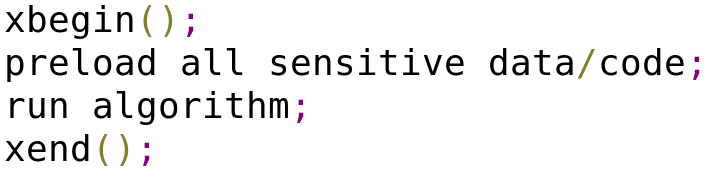
\includegraphics[scale=0.25]{images/cloakcode}
	\caption{Cloak sample code \cite{cloak}}
	\label{alg:cloak}
\end{algorithm}

For preloading, if the attacker targets L1, the code should be preloaded into L1-I by execution. Also, all the data should be loaded into the write set. For the attackers targeting L3, code and read-only data should be loaded into read set, while the data which will possibly be touched again should be loaded into the write set \cite{cloak}.

%The evaluation of this work has been done by running weak implementations of existing algorithms in enclave secured by the implementation of this research, named Cloak. The AES T-table implementation of OpenSSL which is known to be vulnerable to cache attacks, recovering cryptographic keys and randomly generated numbers by execution path monitoring, RSA square and multiply example and GTK keystroke example which are discussed in the paper are among the attacks used for evaluating the defense method proposed in the paper.

\subsubsection{Analysis}
There will still be some leakage remaining which this research does not handle. Overall execution time can leak information. Also, aborts do not cause the concurrent memory accesses to be canceled. Branch predictor is influenced due to the cache pinning and other micro-architecture effects can be possible due to the modifications to the execution behavior.

The strength of the research is to introduce a new software-based way for pinning data into cache lines which has not been done before. Making use of Intel TSX instructions for this purpose is a novel idea that can be used in various areas other than enclave side channel attack protection. There is also an opportunity for later research on optimization and performance improvement and architectural study for reducing faults.

\subsection{Déjà Vu}
Chen et al. \cite{dejavu} focus on detecting SGX side-channel attacks performed by privileged attackers (OS, etc.). They make use of Intel TSX to embed a clock inside the enclave. The use of TSX is for detecting any interrupts to the clock itself if occurred. When the execution time of the program inside the enclave exceeds a fixed amount of time as the threshold, it is considered that the code has been interrupted by some external factor and an AEX (asynchronous enclave exit) will be detected. Thus, the research claims to detect attacks to a good degree and the evaluation results show little performance overhead and good precision in detecting the attacks.

The implemented clock should be hidden from the OS in terms of reading and modification and it should not be decreased under any condition. These can be assured by implementation inside SGX enclave. Also, the clock should not be stopped or interrupted by the OS. This feature is addressed by using Intel transactional memory. For protecting the clock to be read by the OS, a random value will be generated in a transaction and will be added to the global timer variable. This will run in a thread parallel to the main program which is targeted to be executed inside the enclave.

For measuring the threshold for program interruption detection by the attacker, the system needs to be trained with execution to learn the execution time without AEXs and the minimum time of an AEX execution.

The security evaluation has been done by running attacks on the clock for stopping it, triggering page-faults for tracing the execution, and slowing the clock by modifying CPU cores' working frequency.

%Performance evaluation of this work is done by running nbench benchmark algorithms and measuring the normalized execution time of them.

\begin{figure}
	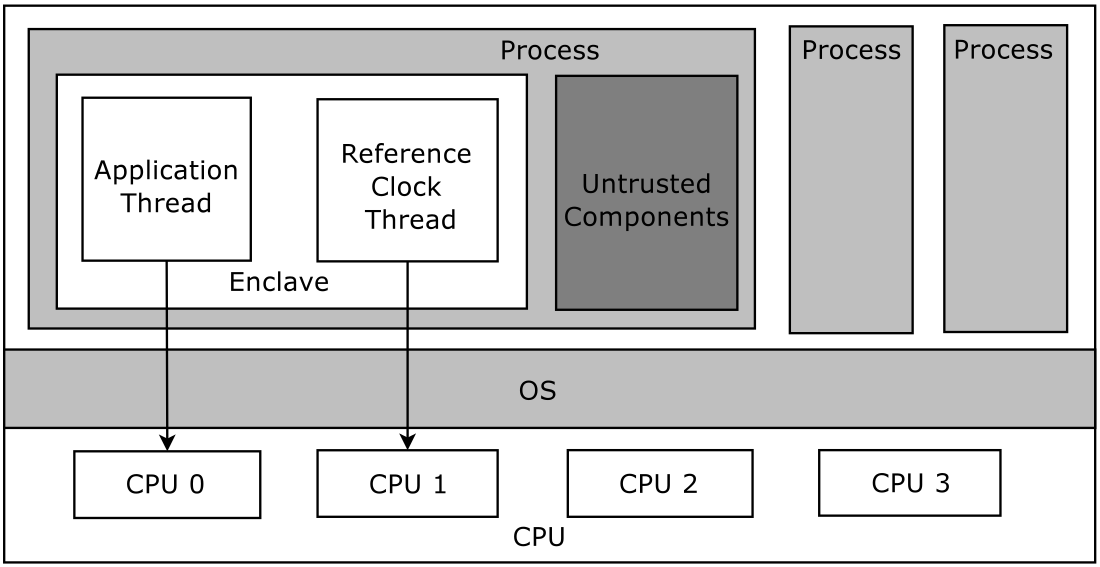
\includegraphics[scale=0.2]{images/dejavu}
	\caption{System architecture of Déjà Vu. Blocks in gray are untrusted, which include the untrusted components of the processes and the entire OS kernel \cite{dejavu}.}
	\label{fig:dejavu}
\end{figure}

\subsubsection{Strengths and Weaknesses}
The problem with this method is that it only considers enclave exits as points of attacks and possible attacks that may have been occurred during the execution which do not cause AEX have been excluded. So, attacks like B-SPM and HT-SPM (sneaky page monitoring attacks in general) which do not rely on AEX can still be effective in the presence of Déjà Vu.

\subsection{Pigeonhole attacks}
Shinde et al. \cite{pigeonhole} study the possible side-channel attacks which make use of page-faults. Firstly, they do a statistical study on the percent of leakage, vulnerability, and the possibility and effectiveness of page-fault based attacks which they call pigeonhole attacks. Then, they study the possible ways of eliminating page-fault side-channels. The paper claims that for lowering the overheads, there is a need for hardware changes. It defines pigeonhole attack as an attack that is performed when a page table walk is done. Moving data between physical memory and virtual memory from different pages sequentially causes page-faults on every single page when the virtual memory is already full, holding all the other pages. When the first page is fetched, the next page will be removed from the page table and when the next page is to be fetched, a page fault will occur.

The solution of the paper is based on the fact that the malicious OS cannot differentiate accesses which are occurred in a single page. Thus, by mapping all the input dependent data into a single page, the program will access the same pattern of the pages independent of the input and makes it page fault oblivious. The page containing the input dependent data is called data staging page and the page containing the code is called code staging page. By creating a decision tree of the program instructions, it is understood that in each stage of the program which is being executed, there is a page-fault sequence dependent on the data, which can be mapped to a staging page. So for each stage, we consider a staging page.

This technique will create a big overhead, thus the paper also works on optimizing the method they have implemented. The optimizations are:
\begin{itemize}
	\item Eliminating copy operations by skipping saving the read-only data
	\item Merge small data blocks into single pages to reduce the number of fetches
	\item Merge levels of execution and reduce the number of stages
	\item Removing the mux based on the input to reduce the possibility of branch conditions
	\item Remove the dependence of code on the data, Ex. CAS obliviousness
\end{itemize}

The idea of the paper has been implemented as an LLVM compiler pass.

\subsection{Stealthy}
This paper introduces a new group of side-channel attacks named stealthy page table-based attacks which are not dependent on page faults and can recover useful information from the data which is being accessed by the program running inside the enclave without page faults being occurred. While current defenses are all based on preventing page faults from happening, there is little effort to prevent attacks which do not depend on page faults.

One of the attack vectors discussed by this paper is pages accessed and dirty bits. Suppose a program is being executed in the enclave which branches based on a secret. If the branch occurs one page will be retrieved and thus its accessed flag will be set, otherwise the same happens for another page. By observing the accessed bit for these two page tables, the secret is revealed. Doing this sequentially can reveal all the secrets which lead to EdDSA session key to be revealed gradually.

The evaluation of this research is done by writing a microbenchmark for measuring interrupts frequency and latency and launching attacks against Libgcrypt EdDSA for extracting private session keys. The results show that it is possible to recover the same session keys which are possible by attacking using page faults without incurring page faults.

\subsubsection{Strengths and Weaknesses}

Does not work on performance optimization but only to attack and recover information without the use of page faults.

\section{SGX-Shield}



\section{Conclusions}

In this article, we develop the first multifrequency MAC protocol for
WSN applications in which each device adopts a
single radio transceiver. The different MAC design requirements for
WSNs and general wireless ad-hoc networks are
compared, and a complete WSN multifrequency MAC design (MMSN) is
put forth. During the MMSN design, we analyze and evaluate different
choices for frequency assignments and also discuss the nonuniform
back-off algorithms for the slotted media access design.

% Start of "Sample References" section

\section{Typical References in New ACM Reference Format}
A paginated journal article \cite{Abril07}, an enumerated
journal article \cite{Cohen07}, a reference to an entire issue \cite{JCohen96},
a monograph (whole book) \cite{Kosiur01}, a monograph/whole book in a series (see 2a in spec. document)
\cite{Harel79}, a divisible-book such as an anthology or compilation \cite{Editor00}
followed by the same example, however we only output the series if the volume number is given
\cite{Editor00a} (so Editor00a's series should NOT be present since it has no vol. no.),
a chapter in a divisible book \cite{Spector90}, a chapter in a divisible book
in a series \cite{Douglass98}, a multi-volume work as book \cite{Knuth97},
an article in a proceedings (of a conference, symposium, workshop for example)
(paginated proceedings article) \cite{Andler79}, a proceedings article
with all possible elements \cite{Smith10}, an example of an enumerated
proceedings article \cite{VanGundy07},
an informally published work \cite{Harel78}, a doctoral dissertation \cite{Clarkson85},
a master's thesis: \cite{anisi03}, an online document / world wide web
resource \cite{Thornburg01, Ablamowicz07, Poker06}, a video game (Case 1) \cite{Obama08} and (Case 2) \cite{Novak03}
and \cite{Lee05} and (Case 3) a patent \cite{JoeScientist001},
work accepted for publication \cite{rous08}, 'YYYYb'-test for prolific author
\cite{SaeediMEJ10} and \cite{SaeediJETC10}. Other cites might contain
'duplicate' DOI and URLs (some SIAM articles) \cite{Kirschmer:2010:AEI:1958016.1958018}.
Boris / Barbara Beeton: multi-volume works as books
\cite{MR781536} and \cite{MR781537}.

A couple of citations with DOIs: \cite{2004:ITE:1009386.1010128,
  Kirschmer:2010:AEI:1958016.1958018}.

Online citations: \cite{TUGInstmem, Thornburg01, CTANacmart}.

% Appendix
\appendix
\section{Switching Times}

In this appendix, we measure the channel switching time of Micaz
\cite{CROSSBOW} sensor devices.  In our experiments, one mote
alternatingly switches between Channels~11 and~12. Every time after
the node switches to a channel, it sends out a packet immediately and
then changes to a new channel as soon as the transmission is finished.
We measure the number of packets the test mote can send in 10 seconds,
denoted as $N_{1}$. In contrast, we also measure the same value of the
test mote without switching channels, denoted as $N_{2}$. We calculate
the channel-switching time $s$ as
\begin{displaymath}%
s=\frac{10}{N_{1}}-\frac{10}{N_{2}}.
\end{displaymath}%
By repeating the experiments 100 times, we get the average
channel-switching time of Micaz motes: 24.3\,$\mu$s.

\section{Supplementary Materials}


\begin{printonly}
  See the supplementary materials in the online version
\end{printonly}

\begin{screenonly}
\subsection{This is an Example of Appendix Subsection Head}

Channel-switching time is measured as the time length it takes for
motes to successfully switch from one channel to another. This
parameter impacts the maximum network throughput, because motes
cannot receive or send any packet during this period of time, and it
also affects the efficiency of toggle snooping in MMSN, where motes
need to sense through channels rapidly.

By repeating experiments 100 times, we get the average
channel-switching time of Micaz motes: 24.3 $\mu$s. We then conduct
the same experiments with different Micaz motes, as well as
experiments with the transmitter switching from Channel 11 to other
channels. In both scenarios, the channel-switching time does not have
obvious changes. (In our experiments, all values are in the range of
23.6 $\mu$s to 24.9 $\mu$s.)

\subsection{Appendix Subsection Head}

The primary consumer of energy in WSNs is idle listening. The key to
reduce idle listening is executing low duty-cycle on nodes. Two
primary approaches are considered in controlling duty-cycles in the
MAC layer.

\end{screenonly}

\begin{acks}

The authors would like to thank Dr. Maura Turolla of Telecom
Italia for providing specifications about the application scenario.

The work is supported by the \grantsponsor{GS501100001809}{National
  Natural Science Foundation of
  China}{http://dx.doi.org/10.13039/501100001809} under Grant
No.:~\grantnum{GS501100001809}{61273304\_a}
and~\grantnum[http://www.nnsf.cn/youngscientists]{GS501100001809}{Young
  Scientists' Support Program}.


\end{acks}

% Bibliography
\bibliographystyle{ACM-Reference-Format}
\bibliography{bibliography}
